\documentclass[a4paper, 12pt]{article}

% ~~~~~~~~~~~~~~~~~~~~~~~~~~~~~~~~~~~~~~~~
% ~~~~~~~~~~~~~~~ PACKAGES ~~~~~~~~~~~~~~~
% ~~~~~~~~~~~~~~~~~~~~~~~~~~~~~~~~~~~~~~~~

\usepackage{amsmath}
\usepackage{relsize}
\usepackage{tikz}
\usepackage{xcolor}
\usetikzlibrary{arrows}

% ~~~~~~~~~~~~~~~~~~~~~~~~~~~~~~~~~~~~~~~~
% ~~~~~~~~~~~~~~~ PREAMBLE ~~~~~~~~~~~~~~~
% ~~~~~~~~~~~~~~~~~~~~~~~~~~~~~~~~~~~~~~~~

\title{Demo Document No. 1\\[0.4em]\smaller{for the SEPTeX module}}
\author{Marcel Simader}
\date{}
\pagenumbering{gobble}
% This is indeed a comment in the preamble

% ~~~~~~~~~~~~~~~~~~~~~~~~~~~~~~~~~~~~
% ~~~~~~~~~~~~~~~ BODY ~~~~~~~~~~~~~~~
% ~~~~~~~~~~~~~~~~~~~~~~~~~~~~~~~~~~~~

\begin{document}
	\maketitle
	
	\noindent This is some text, and it contains a potentially % confusing comment for the "soft" line wrap % functionality
	
	And this is some text that goes on and on and on and on and on and on and on and on and on and on and on and on and on 
		and on and on and on and on and on and on and on and on\ldots
	This is a \LaTeX\ sentence -- wow!
	\begin{gather*}
		\left[ 1, \frac{1}{3}, 3, \text{abc} \right]
		\left\{ 1, -\frac{2}{7}, -\frac{3}{5}, abc \right\}
		\\
		\left( \left\{ 1, 2, 3, -\frac{9}{2} \right\}, \text{addition} \right)
		\left( \left\{ 1, 2, 3, -\frac{9}{2} \right\}, \text{addition}, \text{addition} \right)
	\end{gather*}
	
	\newpage
	
	\begin{figure}[h!]
		\begin{center}
			
\begin{tikzpicture}[draw]
				\definecolor{RED}{RGB}{252, 68, 68}
				\definecolor{ORANGE}{RGB}{255, 165, 0}
				\definecolor{YELLOW}{RGB}{251, 219, 4}
				\definecolor{GREEN}{RGB}{139, 195, 74}
				\definecolor{LIGHT_BLUE}{RGB}{3, 169, 244}
				\definecolor{DARK_BLUE}{RGB}{4, 60, 140}
				\definecolor{PURPLE}{RGB}{103, 58, 183}
				\definecolor{MAGENTA}{RGB}{156, 39, 176}
				\definecolor{PINK}{RGB}{236, 76, 140}
				\definecolor{ROSE}{RGB}{252, 140, 132}
				\definecolor{ALMOST_BLACK}{RGB}{18, 18, 18}
				\definecolor{DARK_GRAY}{RGB}{45, 45, 45}
				\definecolor{LIGHT_GRAY}{RGB}{180, 180, 180}
				\definecolor{ALMOST_WHITE}{RGB}{245, 245, 245}
				\begin{scope}[draw, scale={0.4}]
					\draw[draw, line width={0.5mm}, color={ALMOST_BLACK}, fill={RED}] ( 0.000,  0.000) -- ( 4.000,  4.000) 
						-- ( 0.000,  4.000) -- (-4.000,  2.000) -- cycle;
				\end{scope}
				
				\begin{scope}[draw, scale={0.45}]
					\draw[draw, line width={0.5714285714285714mm}, color={ALMOST_BLACK}, fill={ORANGE}] ( 0.000,  1.000) 
						-- ( 4.000,  5.000) -- ( 0.000,  5.000) -- (-4.000,  3.000) -- cycle;
				\end{scope}
				
				\begin{scope}[draw, scale={0.5}]
					\draw[draw, line width={0.6428571428571428mm}, color={ALMOST_BLACK}, fill={YELLOW}] ( 0.000,  2.000) 
						-- ( 4.000,  6.000) -- ( 0.000,  6.000) -- (-4.000,  4.000) -- cycle;
				\end{scope}
				
				\begin{scope}[draw, scale={0.55}]
					\draw[draw, line width={0.7142857142857143mm}, color={ALMOST_BLACK}, fill={GREEN}] ( 0.000,  3.000) -- 
						( 4.000,  7.000) -- ( 0.000,  7.000) -- (-4.000,  5.000) -- cycle;
				\end{scope}
				
				\begin{scope}[draw, scale={0.6}]
					\draw[draw, line width={0.7857142857142857mm}, color={ALMOST_BLACK}, fill={LIGHT_BLUE}] ( 0.000,  4.000) 
						-- ( 4.000,  8.000) -- ( 0.000,  8.000) -- (-4.000,  6.000) -- cycle;
				\end{scope}
				
				\begin{scope}[draw, scale={0.65}]
					\draw[draw, line width={0.8571428571428572mm}, color={ALMOST_BLACK}, fill={DARK_BLUE}] ( 0.000,  5.000) 
						-- ( 4.000,  9.000) -- ( 0.000,  9.000) -- (-4.000,  7.000) -- cycle;
				\end{scope}
				
				\begin{scope}[draw, scale={0.7}]
					\draw[draw, line width={0.9285714285714286mm}, color={ALMOST_BLACK}, fill={PURPLE}] ( 0.000,  6.000) 
						-- ( 4.000,  10.000) -- ( 0.000,  10.000) -- (-4.000,  8.000) -- cycle;
				\end{scope}
				
				\begin{scope}[draw, scale={0.75}]
					\draw[draw, line width={1.0mm}, color={ALMOST_BLACK}, fill={MAGENTA}] ( 0.000,  7.000) -- ( 4.000,  11.000) 
						-- ( 0.000,  11.000) -- (-4.000,  9.000) -- cycle;
				\end{scope}
				
				\begin{scope}[draw, scale={0.8}]
					\draw[draw, line width={1.0714285714285714mm}, color={ALMOST_BLACK}, fill={PINK}] ( 0.000,  8.000) -- 
						( 4.000,  12.000) -- ( 0.000,  12.000) -- (-4.000,  10.000) -- cycle;
				\end{scope}
				
				\begin{scope}[draw, scale={0.8500000000000001}]
					\draw[draw, line width={1.1428571428571428mm}, color={ALMOST_BLACK}, fill={ROSE}] ( 0.000,  9.000) -- 
						( 4.000,  13.000) -- ( 0.000,  13.000) -- (-4.000,  11.000) -- cycle;
				\end{scope}
				
				\begin{scope}[draw, scale={0.9}]
					\draw[draw, line width={1.2142857142857144mm}, color={ALMOST_BLACK}, fill={ALMOST_BLACK}] ( 0.000,  10.000) 
						-- ( 4.000,  14.000) -- ( 0.000,  14.000) -- (-4.000,  12.000) -- cycle;
				\end{scope}
				
				\begin{scope}[draw, scale={0.95}]
					\draw[draw, line width={1.2857142857142856mm}, color={ALMOST_BLACK}, fill={DARK_GRAY}] ( 0.000,  11.000) 
						-- ( 4.000,  15.000) -- ( 0.000,  15.000) -- (-4.000,  13.000) -- cycle;
				\end{scope}
				
				\begin{scope}[draw, scale={1.0}]
					\draw[draw, line width={1.3571428571428572mm}, color={ALMOST_BLACK}, fill={LIGHT_GRAY}] ( 0.000,  12.000) 
						-- ( 4.000,  16.000) -- ( 0.000,  16.000) -- (-4.000,  14.000) -- cycle;
				\end{scope}
				
				\begin{scope}[draw, scale={1.05}]
					\draw[draw, line width={1.4285714285714286mm}, color={ALMOST_BLACK}, fill={ALMOST_WHITE}] ( 0.000,  13.000) 
						-- ( 4.000,  17.000) -- ( 0.000,  17.000) -- (-4.000,  15.000) -- cycle;
				\end{scope}
				
			\end{tikzpicture}
			
		\end{center}
		
		\caption{Captions, Figures, and the Default Colors.}
	\end{figure}
	
	\newpage
	
	\begin{figure}[h!]
		\begin{center}
			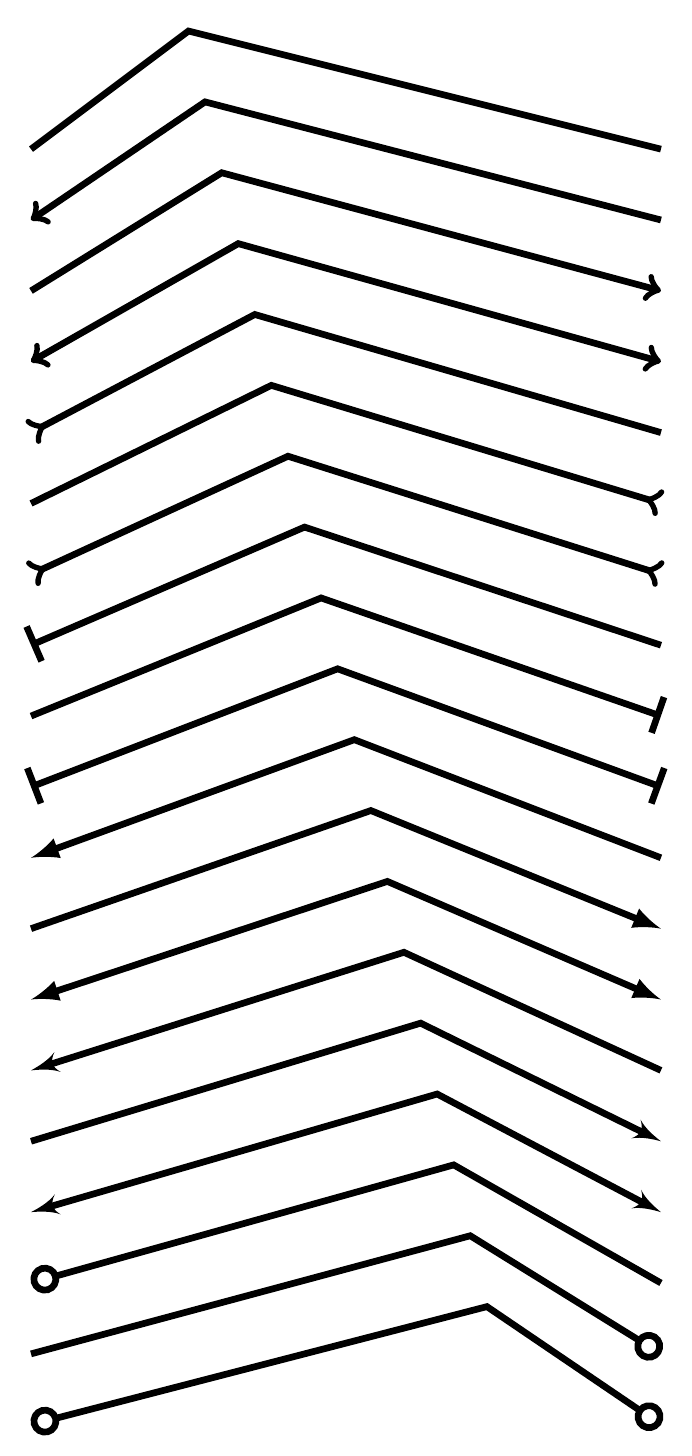
\begin{tikzpicture}[draw]
				\begin{scope}[draw, scale={2}, shift={(0, 0.0)}]
					\draw[-, draw, line width={0.85mm}] ( 0.000,  0.000) to ( 1.000,  0.750) to ( 4.000,  0.000);
				\end{scope}
				
				\begin{scope}[draw, scale={2}, shift={(0, -0.45)}]
					\draw[<-, draw, line width={0.85mm}] ( 0.000,  0.000) to ( 1.105,  0.750) to ( 4.000,  0.000);
				\end{scope}
				
				\begin{scope}[draw, scale={2}, shift={(0, -0.9)}]
					\draw[->, draw, line width={0.85mm}] ( 0.000,  0.000) to ( 1.211,  0.750) to ( 4.000,  0.000);
				\end{scope}
				
				\begin{scope}[draw, scale={2}, shift={(0, -1.35)}]
					\draw[<->, draw, line width={0.85mm}] ( 0.000,  0.000) to ( 1.316,  0.750) to ( 4.000,  0.000);
				\end{scope}
				
				\begin{scope}[draw, scale={2}, shift={(0, -1.8)}]
					\draw[>-, draw, line width={0.85mm}] ( 0.000,  0.000) to ( 1.421,  0.750) to ( 4.000,  0.000);
				\end{scope}
				
				\begin{scope}[draw, scale={2}, shift={(0, -2.25)}]
					\draw[-<, draw, line width={0.85mm}] ( 0.000,  0.000) to ( 1.526,  0.750) to ( 4.000,  0.000);
				\end{scope}
				
				\begin{scope}[draw, scale={2}, shift={(0, -2.7)}]
					\draw[>-<, draw, line width={0.85mm}] ( 0.000,  0.000) to ( 1.632,  0.750) to ( 4.000,  0.000);
				\end{scope}
				
				\begin{scope}[draw, scale={2}, shift={(0, -3.15)}]
					\draw[|-, draw, line width={0.85mm}] ( 0.000,  0.000) to ( 1.737,  0.750) to ( 4.000,  0.000);
				\end{scope}
				
				\begin{scope}[draw, scale={2}, shift={(0, -3.6)}]
					\draw[-|, draw, line width={0.85mm}] ( 0.000,  0.000) to ( 1.842,  0.750) to ( 4.000,  0.000);
				\end{scope}
				
				\begin{scope}[draw, scale={2}, shift={(0, -4.05)}]
					\draw[|-|, draw, line width={0.85mm}] ( 0.000,  0.000) to ( 1.947,  0.750) to ( 4.000,  0.000);
				\end{scope}
				
				\begin{scope}[draw, scale={2}, shift={(0, -4.5)}]
					\draw[latex-, draw, line width={0.85mm}] ( 0.000,  0.000) to ( 2.053,  0.750) to ( 4.000,  0.000);
				\end{scope}
				
				\begin{scope}[draw, scale={2}, shift={(0, -4.95)}]
					\draw[-latex, draw, line width={0.85mm}] ( 0.000,  0.000) to ( 2.158,  0.750) to ( 4.000,  0.000);
				\end{scope}
				
				\begin{scope}[draw, scale={2}, shift={(0, -5.4)}]
					\draw[latex-latex, draw, line width={0.85mm}] ( 0.000,  0.000) to ( 2.263,  0.750) to ( 4.000,  0.000);
				\end{scope}
				
				\begin{scope}[draw, scale={2}, shift={(0, -5.8500000000000005)}]
					\draw[latex'-, draw, line width={0.85mm}] ( 0.000,  0.000) to ( 2.368,  0.750) to ( 4.000,  0.000);
				\end{scope}
				
				\begin{scope}[draw, scale={2}, shift={(0, -6.3)}]
					\draw[-latex', draw, line width={0.85mm}] ( 0.000,  0.000) to ( 2.474,  0.750) to ( 4.000,  0.000);
				\end{scope}
				
				\begin{scope}[draw, scale={2}, shift={(0, -6.75)}]
					\draw[latex'-latex', draw, line width={0.85mm}] ( 0.000,  0.000) to ( 2.579,  0.750) to ( 4.000,  0.000);
				\end{scope}
				
				\begin{scope}[draw, scale={2}, shift={(0, -7.2)}]
					\draw[o-, draw, line width={0.85mm}] ( 0.000,  0.000) to ( 2.684,  0.750) to ( 4.000,  0.000);
				\end{scope}
				
				\begin{scope}[draw, scale={2}, shift={(0, -7.65)}]
					\draw[-o, draw, line width={0.85mm}] ( 0.000,  0.000) to ( 2.789,  0.750) to ( 4.000,  0.000);
				\end{scope}
				
				\begin{scope}[draw, scale={2}, shift={(0, -8.1)}]
					\draw[o-o, draw, line width={0.85mm}] ( 0.000,  0.000) to ( 2.895,  0.750) to ( 4.000,  0.000);
				\end{scope}
				
			\end{tikzpicture}
			
		\end{center}
		
		\caption{The arrow styles.}
	\end{figure}
	
	\newpage
	
	\begin{figure}[h!]
		\begin{center}
			\begin{tikzpicture}[draw]
				\node[draw, circle] (x11) at (-2.500,  4.330) {11};
				\node[draw, circle] (x0) at ( 0.000,  5.000) {0};
				\draw[-latex', draw, dashed, bend left={15}, line width={0.3mm}] (x11) to (x0);
				\node[draw, circle] (x1) at ( 2.500,  4.330) {1};
				\draw[-latex', draw, dashed, bend left={15}, line width={0.3mm}] (x0) to (x1);
				\node[draw, circle] (x2) at ( 4.330,  2.500) {2};
				\draw[-latex', draw, dashed, bend left={15}, line width={0.3mm}] (x1) to (x2);
				\node[draw, circle] (x3) at ( 5.000,  0.000) {3};
				\draw[-latex', draw, dashed, bend left={15}, line width={0.3mm}] (x2) to (x3);
				\node[draw, circle] (x4) at ( 4.330, -2.500) {4};
				\draw[-latex', draw, dashed, bend left={15}, line width={0.3mm}] (x3) to (x4);
				\node[draw, circle] (x5) at ( 2.500, -4.330) {5};
				\draw[-latex', draw, dashed, bend left={15}, line width={0.3mm}] (x4) to (x5);
				\node[draw, circle] (x6) at ( 0.000, -5.000) {6};
				\draw[-latex', draw, dashed, bend left={15}, line width={0.3mm}] (x5) to (x6);
				\node[draw, circle] (x7) at (-2.500, -4.330) {7};
				\draw[-latex', draw, dashed, bend left={15}, line width={0.3mm}] (x6) to (x7);
				\node[draw, circle] (x8) at (-4.330, -2.500) {8};
				\draw[-latex', draw, dashed, bend left={15}, line width={0.3mm}] (x7) to (x8);
				\node[draw, circle] (x9) at (-5.000, -0.000) {9};
				\draw[-latex', draw, dashed, bend left={15}, line width={0.3mm}] (x8) to (x9);
				\node[draw, circle] (x10) at (-4.330,  2.500) {10};
				\draw[-latex', draw, dashed, bend left={15}, line width={0.3mm}] (x9) to (x10);
				\draw[-latex', draw, dashed, bend left={15}, line width={0.3mm}] (x10) to (x11);
				\draw[-o, draw] (x0) to (x7);
			\end{tikzpicture}
			
		\end{center}
		
		\caption{Nodes, nodes, nodes.}
	\end{figure}
	
\end{document}